\chapter{Problem}
describe each problem i encountered in detail and how to solve them

\section{MOSFET Convergence Issus}
\emph{problem description:}
\newline
In current model, whether the MOSFET will converge highly depends on the initial state. Under 1.8V Vdd, in most cases encountered, if set the initial of Vgs to 1.8v for nmos and -1.8V for pmos and Vds to 0, the model have no problem of convergence(the test case is pesudo-nmos/pmos inverter, and this setting is essentially set the initial condition to linear region)
\newline
however, if set the initial condition to saturation region, (or in the inverter case, set all the value to 0, and after one iteration, it will become in saturation region), the circuit seems never be able to converge. A more detailcheck shows that in iterations, vds will get smaller and smaller(negative). this error are illustrate in the figure below
\begin{figure}[t!]
\centering
\begin{minipage}[t]{0.5\textwidth}
	\centering
	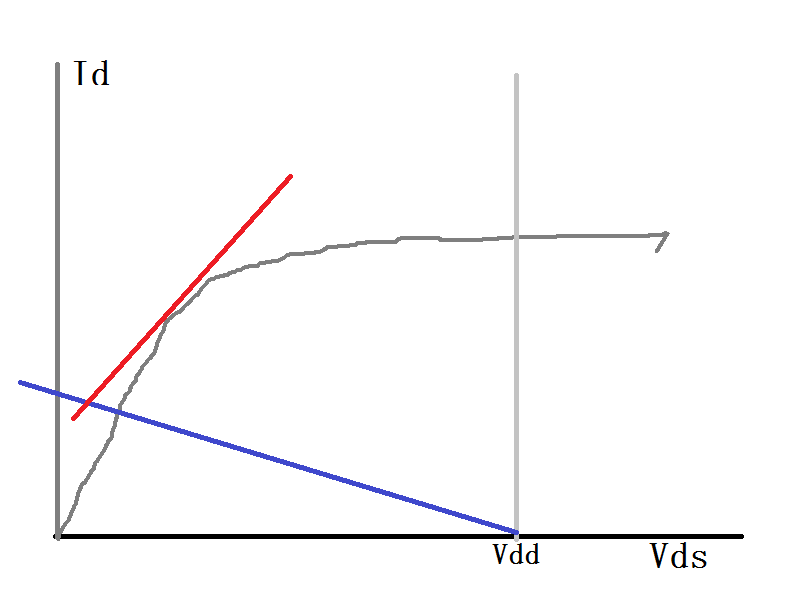
\includegraphics[width=0.4\textwidth]{../figures/mos_converge_normal.png}
	\caption{Unfold in Linear Region}
\end{minipage}
\begin{minipage}[t]{0.5\textwidth}
	\centering
	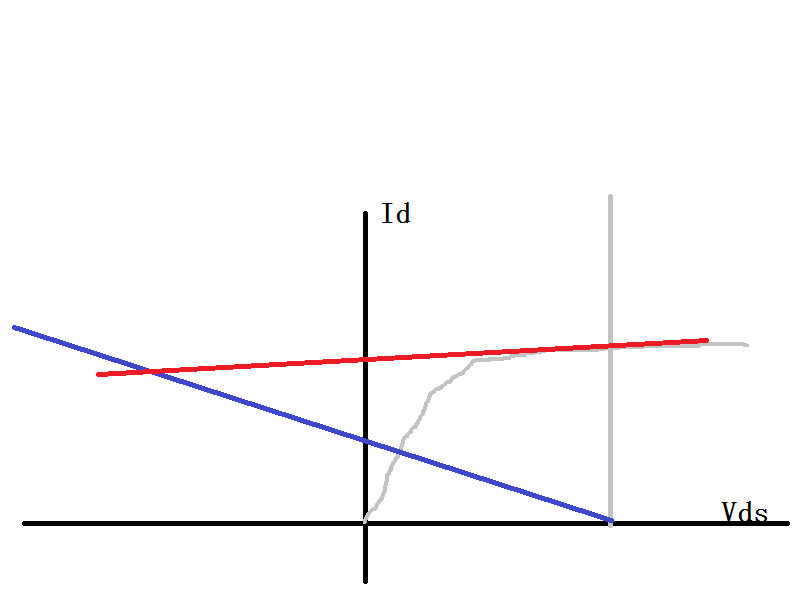
\includegraphics[width=0.4\textwidth]{../figures/mos_converge_abnormal.png}
	\caption{Unfold in Saturation Region}
\end{minipage}
\end{figure}
 the reason why unfold in saturation region will lead to an Unconvergence Issue is that current mosfet model can't cover the behavior in the negative Vds plane, and actuall using the model for the positive plane will lead the next iteration to even further, thus result in never ever will converge.
 \subsubsection{temporary remedy}
 a way to deal this is to force the Vds out of the negative plane(for pmos, keep it out of positive plane). to do so , ever time doing iteration, if find the vds falls in the negative plane, just set it to 0. This method prove to work out fine.
